\documentclass[conference]{IEEEtran}
\usepackage{graphicx}
\usepackage{cite}
\usepackage{amsmath, amssymb}
\usepackage{url}
\usepackage{algorithm}
\usepackage{algorithmic}
\usepackage{booktabs}
\usepackage{multirow}
\usepackage[dvipsnames]{xcolor}
\usepackage{tikz}
\usetikzlibrary{positioning, arrows.meta, calc, fit, backgrounds}

\title{Hybrid Deep Reinforcement Learning and LQR Framework for Rover Path Tracking in Dynamic Terrain}
\author{Aaron Sharp, Dang Tran, Hongsheng He}
\date{2026}

\begin{document}
\maketitle

\begin{abstract}
Robotic trajectory control on Mars presents significant challenges due to unstable, deformable, and uncertain terrain. Traditional trajectory-tracking methods rely on structured models that struggle with rapidly varying wheel--terrain interactions such as slip and sinkage. This paper presents a hybrid control framework that integrates deep reinforcement learning (DRL) with a linear quadratic regulator (LQR) for path tracking on dynamic terrain. The LQR provides a stable, interpretable baseline that produces velocity references and corrective feedback, while a Proximal Policy Optimization (PPO) residual policy adapts to terrain-induced disturbances that the linear model cannot capture. We train in a GPU-accelerated, massively parallel simulator (NVIDIA Isaac Sim / Isaac Lab) that simulates thousands of rovers in parallel and couples training to an automatic domain-randomization (ADR) terrain curriculum. We evaluate three controllers, pure LQR, pure PPO, and the hybrid, under identical, matched terrain, friction, and path conditions so that the controller is the only independent variable, and we report cross-track error, slip, sample efficiency, and task-completion (success) rate. The framework is assessed in large-scale simulation and on a physical differential-drive Leo Rover in sand-like terrain. This work is motivated by the long-term goal of enabling multi-robot collaboration on Mars for cooperative tasks such as transporting large rocks or conducting science missions.
\end{abstract}

\section{Introduction}
Uncrewed Ground Vehicles (UGVs) are increasingly deployed in unstructured off-road domains including planetary exploration, mining, and remote science operations, where vehicles must negotiate highly variable terrain such as slopes, rocks, and deformable soils. Precise motion planning and closed-loop tracking on such terrains is challenging due to complex and often poorly modeled wheel--terrain interactions that produce slip, sinkage, and rapidly varying dynamics \cite{mehta2024hybrid, wiberg2021rough, bekker1969introduction}.

Classical model-based controllers (e.g., PID, LQR, MPC) are advantageous for their interpretability and performance under nominal conditions. LQR-type controllers provide efficient linear feedback and provable stability about an operating point, and MPC provides constraint handling and planning; however, both rely on accurate models and can suffer when vehicle--soil contact dynamics become strongly nonlinear or time-varying, as occurs on deformable granular surfaces. Moreover, MPC's online computational demands and dependency on model fidelity complicate deployment on resource-constrained planetary platforms \cite{zhang2023energy, mehta2024hybrid}.

Model-free Deep Reinforcement Learning (DRL) methods (e.g., PPO \cite{schulman2017proximal}, SAC) can learn complex control mappings that implicitly compensate for unmodeled dynamics and perceptual uncertainty, and have shown promising performance for locomotion and rough-terrain tasks \cite{wiberg2021rough, gunma2024sac, lee2020learning}. However, purely end-to-end DRL approaches are often sample-inefficient, require many millions of environment interactions to converge, and are sensitive to the sim-to-real gap, challenges that are exacerbated when high-fidelity simulation of deformable soils (sand) is computationally expensive or infeasible \cite{blum2020ppmc, mortensen2023teacher}. The advent of GPU-accelerated, massively parallel simulators has substantially relaxed the sample-efficiency barrier by running thousands of environment copies on a single workstation GPU, enabling locomotion policies to be trained in minutes rather than days \cite{makoviychuk2021isaac, rudin2022learning, mittal2023orbit}. Recurrent policy architectures (e.g., LSTM-augmented networks) and training curricula have been demonstrated to mitigate partial observability and improve tracking under temporally-correlated slip dynamics \cite{alcayaga2025lstm}.

Hybrid strategies that combine a model-based baseline with a learned corrective policy (residual or HDRL methods) offer a pragmatic compromise: the classical controller supplies stability and interpretable baseline behavior, while the learned policy focuses on compensating residual errors caused by unmodeled dynamics and environmental uncertainty. Mehta et al. (2024) demonstrated that merging an LQR baseline with a PPO-based DRL residual significantly reduces training instability and improves off-road path tracking for an Ackermann platform compared to purely model-free or purely classical controllers \cite{mehta2024hybrid}. Other hybrid approaches (e.g., sliding-mode control augmented with learned slip estimators) similarly show that learned components can provide effective compensation without abandoning the guarantees of classical controllers \cite{nourizadeh2023sliding}.

Despite these advances, there is a notable gap when the substrate is a strongly deformable granular material (sand-like), where soil mechanics (sinkage, changing normal loads) produce rich dynamics that are expensive to simulate faithfully and difficult to capture with simplified models. The path-planning literature that incorporates terrain-aware costs emphasizes the importance of slope and soil modeling for energy-efficient routing, but planning-focused work does not directly address low-level tracking under transient slip or sinkage events \cite{yang2025dqnt, zhang2023energy}. Similarly, teacher-student and imitation-based strategies provide promising sim-to-real transfer pathways, which are attractive when the collection of real hardware data is limited or costly \cite{mortensen2023teacher, wang2025rov}.

In this work, we propose a hybrid residual controller tailored to a velocity-controlled differential-drive rover operating on dynamic, sand-like terrain. The framework uses an LQR baseline to produce safe, stabilizing velocity references and a PPO-trained residual policy to correct for terrain-induced disturbances (slip, sinkage, transient traction loss). We expect the hybrid approach to (1) reduce the sample complexity and instability commonly associated with end-to-end DRL, (2) provide safer initial behavior during training and early deployment, and (3) increase robustness to terrain parameter variations via domain randomization and an automatic curriculum. The primary contributions of this paper are:
\begin{itemize}
  \item A hybrid LQR + PPO residual architecture adapted for a velocity-controlled rover on deformable, uneven terrain, including state and observation structures appropriate for partial observability and forward terrain sensing.
  \item A GPU-accelerated, massively parallel training pipeline built on NVIDIA Isaac Sim / Isaac Lab, coupled to an automatic domain-randomization (ADR) terrain curriculum that simulates thousands of rovers in parallel and progressively increases terrain difficulty as competence improves.
  \item A controlled evaluation protocol that holds terrain, friction, and reference paths \emph{identical} across pure LQR, pure PPO, and the hybrid (matched random seeds), with discrete path-geometry test sets and slope-logged randomized terrain that enables slope-conditioned analysis.
  \item Comprehensive validation comparing pure classical control, end-to-end DRL, and the hybrid residual approach across cross-track error, slip, sample efficiency, and task-completion rate, in simulation and on a physical Leo Rover in a sand pit.
\end{itemize}

\section{Related Work}
\noindent\textbf{Classical control and model-based planners.} Classical control approaches (PID, LQR, MPC) remain the baseline for many path-following and stability tasks because of their interpretability and computational efficiency. LQR provides compact linear-feedback laws that perform well near a linearization point but can be brittle when wheel--terrain interactions are strongly nonlinear; MPC offers constraint handling and planning at the cost of increased online computation and model dependence \cite{mehta2024hybrid, zhang2023energy}. For deformable, sand-like soils, these methods typically require expensive identification or simplifications that limit performance in the presence of sinkage and time-varying traction \cite{bekker1969introduction, wong2008theory}.

\vspace{2mm}
\noindent\textbf{Model-free DRL and large-scale simulation.} Model-free DRL has been successfully applied to complex locomotion and off-road tasks, demonstrating the ability to compensate for high-dimensional, partially observed dynamics through end-to-end learning \cite{wiberg2021rough, gunma2024sac, lee2020learning}. A key enabler has been GPU-parallel simulation: Isaac Gym \cite{makoviychuk2021isaac} and the Orbit/Isaac Lab framework \cite{mittal2023orbit} run thousands of environments on a single GPU, and Rudin et al. \cite{rudin2022learning} showed that a game-inspired terrain curriculum with massive parallelism can train quadruped locomotion in minutes. These advances directly motivate our use of Isaac Lab for large-scale training. The remaining limitations for our setting are simulator fidelity for granular soils and partial observability of slip; recurrent architectures (e.g., LSTM) have been shown to help under temporally correlated slip conditions \cite{alcayaga2025lstm}.

\vspace{2mm}
\noindent\textbf{Hybrid control and residual learning.} Combining classical controllers with learned residuals has emerged as an effective trade-off: the baseline controller supplies stability and safe behavior, while a learning-based residual compensates for unmodeled effects. Mehta et al. (2024) present an LQR+PPO residual design for Ackermann platforms, which reduces training instability and improves tracking in rough terrain \cite{mehta2024hybrid}. Approaches that integrate learned slip estimators with sliding-mode or other robust controllers similarly improve tracking accuracy while retaining formal control properties \cite{nourizadeh2023sliding}. These hybrid paradigms motivate our choice to use LQR as a stabilizing baseline and a PPO residual learner for deformable terrain.

\vspace{2mm}
\noindent\textbf{Generalization and simulation-to-real strategies.} Several works focus on transferability through curriculum learning, domain randomization \cite{tobin2017domain}, and teacher-student schemes. The PPMC algorithm and related curricula emphasize robust generalization across diverse terrain types \cite{blum2020ppmc}, while teacher-student pipelines demonstrate effective sim-to-real transfer for map-less rover navigation by progressively injecting noise and real-world variability \cite{mortensen2023teacher}. Recent high-fidelity sim-to-real work (e.g., Orsula \textit{et al.}, 2025) uses particle-based granular simulation to train agents that transfer to real sand; such simulators model sinkage and transient traction more faithfully but require extremely large compute (millions of particles, heavy GPU usage) \cite{orsula2025sim2dust}. Imitation-from-observation provides another route to reduce training time when demonstrations are available \cite{wang2025rov}. These strategies inform our domain-randomization and curriculum design.

\vspace{2mm}
\noindent\textbf{Planning, energy, and safety considerations.} Planning works with terrain-aware costs underscore the importance of slope and soil modeling for energy-optimal routing, yet path planning alone does not resolve low-level tracking failures caused by transient sinkage or slip \cite{yang2025dqnt, zhang2023energy}. Safety and clearance estimation (e.g., NASA's ACE concepts) remain critical for planetary deployment and motivate conservative checks combined with the controller during motion execution \cite{nasaACE}.

\vspace{2mm}
\noindent\textbf{Gap addressed by our work.} Taken together, the literature shows that (1) purely classical or purely learned solutions each have important limitations on deformable terrain, (2) recurrent and curriculum-based DRL help but do not eliminate the sim-to-real challenge, and (3) hybrid residual frameworks provide a promising path to safer, sample-efficient learning. Our work leverages these lessons by pairing an LQR baseline (stability and interpretability) with a PPO residual (slip/sinkage compensation), trained at scale in Isaac Lab with an automatic terrain curriculum, and evaluated under a controlled, matched-condition protocol on both simulated and physical platforms.

\section{Proposed Method}
Figure~\ref{fig:architecture} summarizes the hybrid control architecture. A trajectory profiler converts the reference path into per-waypoint reference velocities; the LQR baseline produces a stabilizing velocity/turn-rate command from the tracking error, and the PPO policy adds a bounded residual that compensates for terrain-induced disturbances. The combined command is mapped to wheel velocities and applied to the rover, in simulation or on hardware.

\begin{figure}[t]
\centering
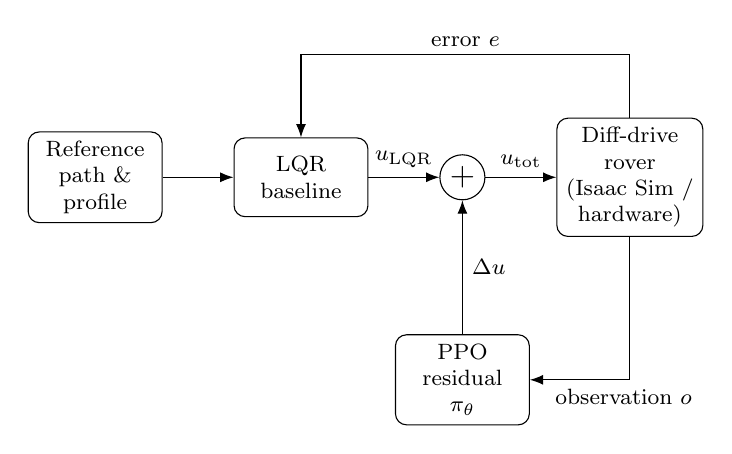
\begin{tikzpicture}[
  font=\footnotesize,
  block/.style={draw, rounded corners, minimum width=1.7cm, minimum height=1.0cm, align=center},
  sum/.style={draw, circle, inner sep=1.5pt},
  >=Latex
]
% --- top row: path -> LQR -> (+) -> rover ---
\node[block] (path) {Reference\\path \&\\profile};
\node[block, right=0.9cm of path] (lqr) {LQR\\baseline};
\node[sum, right=0.9cm of lqr] (sum) {\large$+$};
\node[block, right=0.9cm of sum] (rover) {Diff-drive\\rover\\(Isaac Sim /\\hardware)};
% --- PPO residual well below the summing junction ---
\node[block, below=1.7cm of sum] (ppo) {PPO\\residual\\$\pi_\theta$};

% forward signal path
\draw[->] (path) -- (lqr);
\draw[->] (lqr) -- node[above]{$u_{\text{LQR}}$} (sum);
\draw[->] (sum) -- node[above]{$u_{\text{tot}}$} (rover);

% residual feeds straight up into the sum (clean vertical line)
\draw[->] (ppo) -- node[right]{$\Delta u$} (sum);

% observation feedback: down from rover, then left into the RIGHT side of PPO
\coordinate (obs) at (rover.south |- ppo.east);
\draw[->] (rover.south) -- (obs) -- (ppo.east);
\node[anchor=north west] at ($(ppo.east)+(0.2cm,0)$) {observation $o$};

% error feedback: up from rover, across the top, down into LQR
\draw[->] (rover.north) -- ++(0,0.8) -| (lqr.north);
\node[above, yshift=3pt] at ($(rover.north)!0.5!(lqr.north)+(0,0.8)$) {error $e$};
\end{tikzpicture}
\caption{Hybrid LQR{+}PPO residual control architecture. The LQR baseline guarantees stable, interpretable tracking; the bounded PPO residual $\Delta u$ corrects for slip, sinkage, and other unmodeled terrain effects. Pure-LQR uses only the upper path; pure-PPO replaces the baseline with a direct policy command.}
\label{fig:architecture}
\end{figure}

\subsection{Vehicle Model}
We employ a differential-drive Leo Rover controlled by velocity inputs $u = [v, \omega]^T$, where $v$ is the forward velocity and $\omega$ is the angular velocity. The platform is equipped with an IMU for orientation/acceleration, wheel encoders for velocity estimation, and an XVisio SeerSense DS80 stereo camera for forward terrain perception. The kinematic model follows standard unicycle/differential-drive dynamics:
\begin{align}
\dot{x} &= v \cos(\theta), &
\dot{y} &= v \sin(\theta), &
\dot{\theta} &= \omega,
\end{align}
where $(x, y)$ is the position and $\theta$ is the heading. The commanded body velocity is mapped to left/right wheel angular velocities by the differential-drive relation $\dot{\phi}_{L,R} = (v \mp \omega L)/(2r)$, with wheel base $L = 0.34$~m. Velocity commands are limited to the Leo Rover hardware envelope, $|v| \le 0.4$~m/s and $|\omega| \le 1.047$~rad/s ($\approx 60^\circ$/s). On deformable terrain, slip and sinkage introduce discrepancies between commanded and actual velocities, which we address through the hybrid control framework.

\subsection{LQR Baseline Controller}
The LQR controller stabilizes tracking by regulating a path-frame error state to zero. We use the linearized unicycle error model with state
\begin{equation}
\mathbf{e} = [e_{\text{lat}},\; e_{\theta},\; e_{v}]^T,
\end{equation}
where $e_{\text{lat}}$ is the signed lateral (cross-track) offset, $e_{\theta}$ is the heading error, and $e_{v} = v - v_{\text{ref}}$ is the velocity error relative to the trajectory-profile reference speed $v_{\text{ref}}$. The linearized error dynamics are $\dot{\mathbf{e}} = A\mathbf{e} + B\Delta\mathbf{u}$ with
\begin{equation}
A = \begin{bmatrix} 0 & v_{\text{ref}} & 0 \\ 0 & 0 & 0 \\ 0 & 0 & -1 \end{bmatrix},\quad
B = \begin{bmatrix} 0 & 0 \\ 0 & 1 \\ 1 & 0 \end{bmatrix},
\end{equation}
so that the heading channel actuates lateral error through the forward speed and the velocity channel directly regulates $e_v$. The controller minimizes the quadratic cost
\begin{equation}
J = \int_0^\infty \left(\mathbf{e}^T Q \mathbf{e} + \Delta\mathbf{u}^T R \Delta\mathbf{u}\right) dt,
\end{equation}
with $Q = \mathrm{diag}(10,\,6,\,0.5)$ and $R = \mathrm{diag}(0.5,\,0.8)$, yielding the optimal gain $K = R^{-1}B^T P$, where $P$ solves the continuous-time algebraic Riccati equation. The baseline command is
\begin{equation}
\mathbf{u}_{\text{LQR}} = [v_{\text{ref}},\, \omega_{\text{ref}}]^T - K\mathbf{e}.
\end{equation}
Because $A$ depends on $v_{\text{ref}}$, the gain $K(v_{\text{ref}})$ is gain-scheduled: it is precomputed on a fine grid of reference speeds and interpolated online. This baseline ensures safe operation and provides a stable foundation for DRL training by preventing catastrophic failures during exploration.

\subsection{PPO Residual Policy}
The PPO agent outputs a bounded corrective command $\Delta\mathbf{u}$ that is added to the baseline,
\begin{equation}
\mathbf{u}_{\text{tot}} = \mathbf{u}_{\text{LQR}} + \Delta\mathbf{u}, \qquad
|\Delta v| \le 0.15~\text{m/s},\;\; |\Delta\omega| \le 0.30~\text{rad/s},
\end{equation}
where the residual bounds (38\% of $v_{\max}$ and 29\% of $\omega_{\max}$) keep the learned correction authoritative but subordinate to the stabilizing baseline. In the pure-PPO ablation, the policy instead emits the full command $[v,\omega]$ directly. The combined command is clipped to the hardware envelope before the differential-drive mapping.

\noindent\textbf{Observation.} The policy $\pi_\theta$ receives a proprioceptive-plus-terrain observation:
\begin{align}
\mathbf{o} = \big[ &\, e_{\text{lat}},\, e_{\theta},\, v_{\text{fwd}},\, v_{\text{lat}},\, \Delta x^{b}_{\text{wp}},\, \Delta y^{b}_{\text{wp}}, \nonumber\\
& \underbrace{v_{\text{base}},\, \omega_{\text{base}}}_{\text{hybrid only}},\, g^{b}_{x},\, g^{b}_{y},\, g^{b}_{z},\, \mathbf{s}_{\text{terrain}} \big],
\end{align}
where $v_{\text{fwd}}, v_{\text{lat}}$ are body-frame velocities; $(\Delta x^{b}_{\text{wp}}, \Delta y^{b}_{\text{wp}})$ is the next-waypoint vector in the body frame; $(v_{\text{base}},\omega_{\text{base}})$ is the LQR baseline command (provided only to the hybrid policy so the residual is aware of the baseline it is correcting); $\mathbf{g}^{b}=(g^{b}_x,g^{b}_y,g^{b}_z)$ is the gravity vector projected into the body frame, which encodes the rover's roll/pitch and hence the local terrain tilt under the chassis; and $\mathbf{s}_{\text{terrain}}\in\mathbb{R}^{6}$ contains forward terrain-slope features (longitudinal and cross-path slope) for near ($0$--$0.7$~m), mid ($0.7$--$1.2$~m), and far ($1.2$--$2.0$~m) zones, obtained from a forward, downward-facing height scanner that emulates the stereo camera's terrain lookahead. This yields a $15$-dimensional observation for pure PPO and $17$ for the hybrid. The gravity and terrain-lookahead features give the policy partial observability of slope and upcoming traction changes without requiring direct slip measurement.

\noindent\textbf{Reward.} The reward uses dense shaping to encourage accurate path adherence while limiting excessive control effort and rewarding progress:
\begin{align}
r_t = &-w_{\text{cte}}\, e_{\text{lat}}^2 \;-\; w_{\theta}\, e_{\theta}^2 \;+\; w_{v}\, \rho(e_{\text{lat}})\, v_{\text{fwd}}^{+} \nonumber\\
& -\; w_{\text{sm}}\big(|\Delta v_t| + |\Delta\omega_t|\big) \;+\; w_{p}\, \Delta p_t \nonumber\\
& +\; R_{\text{succ}}\,\mathbb{1}[\text{goal}] \;-\; R_{\text{fail}}\,\mathbb{1}[\text{fail}],
\end{align}
where $\rho(e_{\text{lat}}) = \max\!\big(0,\,1 - |e_{\text{lat}}|/c\big)$ with $c=0.5$~m ramps the forward-speed reward down as the rover leaves the path, $v_{\text{fwd}}^{+}=\max(0,v_{\text{fwd}})$, $\Delta p_t$ is the increment in along-path progress, and the terminal terms reward reaching the goal and penalize failures (cross-track error exceeding $2$~m, stagnation, flips, or timeout). The weights are $w_{\text{cte}}=5$, $w_{\theta}=0.5$, $w_{v}=0.5$, $w_{\text{sm}}=0.5$, $w_{p}=10$, $R_{\text{succ}}=200$, and $R_{\text{fail}}=50$. For the hybrid policy we add a residual-effort penalty $-w_{\text{eff}}\lVert\Delta\mathbf{u}_{\text{norm}}\rVert^2$ with $w_{\text{eff}}=0.5$, which discourages the policy from overriding the stable baseline unnecessarily. The smoothness and residual-effort terms together act as the control-effort/energy regularizer; slip is recorded as an evaluation metric rather than a reward term, and is reduced indirectly through accurate heading and cross-track tracking.

\noindent\textbf{Network architecture.} The actor and critic are separate multilayer perceptrons, each with two hidden layers of $256$ units and ReLU activations, preceded by running observation normalization. The policy is a diagonal Gaussian with a state-independent standard deviation parameterized in log-space (initialized at $\log\sigma=-1.0$, i.e.\ $\sigma\approx0.37$, and bounded below at zero by construction), and is optimized with a KL-adaptive learning-rate schedule (target KL $0.02$). We selected this compact architecture deliberately: the observation is low-dimensional ($15$--$17$) and the action is two-dimensional, so a $2\times256$ MLP provides ample capacity without overfitting or slowing the massively parallel rollouts, while wider or deeper networks gave diminishing returns and slower, less stable convergence in preliminary runs. Because slip is temporally correlated and only partially observed, a recurrent variant (a single GRU/LSTM layer feeding the same MLP heads, following \cite{alcayaga2025lstm}) is a natural extension and is treated as an ablation; the memoryless policy with explicit velocity-error feedback already captures much of the required signal and trains more stably at scale.

\subsection{Simulation Environment}
We build the training environment in NVIDIA Isaac Sim 5.1 with the Isaac Lab framework \cite{mittal2023orbit, makoviychuk2021isaac}. Isaac Lab provides GPU-resident, vectorized physics so that thousands of rover instances advance in parallel; we train with $4096$ parallel environments on a single GPU, which makes the multi-hundred-million-step training budget tractable. Key environment settings are:
\begin{itemize}
\item \textbf{Physics and control rate:} physics step $1/50$~s with a decimation of $10$, giving a $0.2$~s control step; Mars gravity $g = 3.71$~m/s$^2$. Wheels are velocity-controlled.
\item \textbf{Episode configuration:} up to $400$~s ($2000$ control steps) or until the goal is reached, the rover flips, leaves bounds, stagnates, or exceeds the cross-track limit.
\item \textbf{Terrain bank:} a procedurally generated bank of $20$ difficulty levels $\times$ $100$ variations ($2000$ distinct height-field patches), combining Mars-like Gaussian-hill fields with standard sloped, wave, stair, and discrete-obstacle sub-terrains. The bank is generated once and cached.
\item \textbf{Domain randomization:} per-episode randomization of wheel--terrain static and dynamic friction over a configured range (spanning low- to high-traction), and per-episode reassignment of each rover to a randomly drawn terrain patch.
\item \textbf{Forward terrain sensing:} a downward ray-caster ahead of the chassis emulates the stereo camera, producing the near/mid/far slope features used in the observation.
\end{itemize}

Figure~\ref{fig:sim_screenshot} shows a representative view of the parallel training environment.

\begin{figure}[t]
\centering
\fbox{\begin{minipage}[c][3.2cm][c]{0.92\columnwidth}\centering\itshape [PLACEHOLDER: screenshot of the Isaac Sim training environment, showing rovers on procedurally generated Mars-like terrain with reference paths overlaid.]\end{minipage}}
\caption{Parallel rover training environment in NVIDIA Isaac Sim / Isaac Lab.}
\label{fig:sim_screenshot}
\end{figure}

\subsection{Training Protocol}
\label{sec:training}
Rather than a small fixed path library, each episode draws a reference path from a bank of $500$ procedurally generated random curved paths (seeded for reproducibility), with per-segment curvature between $25^\circ$ and $120^\circ$ and a total path length of $10$~m. This continuous variety, rather than a handful of hand-designed shapes, is what drives generalization during training. Training is coupled to an \textbf{automatic domain-randomization (ADR) terrain curriculum}: the terrain-difficulty ceiling starts at $10\%$ and advances by $3\%$ whenever the rolling success rate over a $200$-episode window exceeds $70\%$ with mean cross-track error below $0.10$~m, and regresses by $3\%$ if success drops below $50\%$ or mean cross-track error exceeds $0.50$~m, up to a $100\%$ ceiling. On every reset, each environment is assigned a fresh random terrain patch drawn from $[0, \text{current ceiling}]$, so the fleet continually revisits easy terrain while being pushed toward harder terrain as competence grows.

The policy is optimized with PPO \cite{schulman2017proximal} using a GPU-vectorized on-policy runner. Each update collects $32$ steps per environment ($\approx 131{,}000$ transitions per iteration across $4096$ environments). PPO hyperparameters are: learning rate $1.5\times10^{-4}$ (KL-adaptive), clip range $0.2$, $5$ epochs per update with $4$ minibatches, discount $\gamma=0.99$, GAE $\lambda=0.95$, entropy coefficient $0.001$, value-loss coefficient $0.5$, and gradient-norm clipping at $0.5$. The hybrid residual policy is expected to require substantially fewer interactions to reach a given competence than pure PPO, because the LQR baseline already provides stable, near-feasible behavior from the first step. Episodic reward and length statistics are logged for analysis.

\subsection{Deployment Strategy}
To bridge the sim-to-real gap, we rely on (i) the domain randomization and terrain curriculum above, which expose the policy to a wide range of friction and slope conditions; (ii) the LQR baseline, which supplies safe, interpretable behavior during early deployment and bounds the effect of an imperfect residual; and (iii) safety mechanisms, including emergency-stop conditions on heading error ($>90^\circ$) and wheel-current limits, inspired by NASA ACE clearance evaluation \cite{nasaACE}. We do not use a separate teacher-student distillation stage; the hybrid structure itself provides the stable ``teacher-like'' behavior that residual learning refines.

\section{Experiments}
\subsection{Experimental Design}
\subsubsection{Goals and Research Questions}
The primary objective is to evaluate whether the hybrid LQR+PPO residual controller achieves superior path-following on dynamic terrain compared to its constituent baselines, under conditions that isolate the controller as the only variable. Key research questions:
\begin{itemize}
\item \textbf{RQ1:} Does the hybrid approach achieve lower cross-track error and reduced slip than pure LQR and pure PPO?
\item \textbf{RQ2:} Does the hybrid method converge faster (improved sample efficiency) than pure PPO?
\item \textbf{RQ3:} Is the hybrid controller more robust to terrain variation, in particular does its performance degrade least as a function of terrain slope and friction?
\item \textbf{RQ4:} How does performance vary across discrete path geometries (zig-zag, curved, closed polygon)?
\item \textbf{RQ5:} Does the hybrid controller \emph{complete} more paths, i.e.\ achieve a higher task-success rate, than pure LQR and pure PPO?
\end{itemize}

\subsubsection{Compared Methods}
We compare three controllers, which share the identical vehicle model, observation pipeline, and evaluation conditions, differing only in the control policy:
\begin{enumerate}
\item \textbf{LQR-only:} the deterministic baseline of Section~III-B with fixed, gain-scheduled feedback.
\item \textbf{PPO-only:} an end-to-end policy that outputs $[v,\omega]$ directly, with no LQR baseline.
\item \textbf{LQR+PPO (Hybrid):} our proposed method, where PPO outputs a bounded residual added to the LQR baseline.
\end{enumerate}

\subsection{Simulation Experiments}
\subsubsection{Matched-Condition Comparison}
A central design choice is that all three controllers are evaluated on \emph{exactly the same} episodes. Each evaluation episode is drawn from a fixed, ordered list of scenarios that pins the reference path, the terrain patch, and the initial pose, so these are identical across LQR, PPO, and hybrid; the wheel--terrain friction is held at a single controlled level per evaluation run (swept across runs to probe traction sensitivity) rather than randomized per episode, so it too is identical across controllers. Consequently any difference in outcome is attributable to the controller alone, and we can apply paired statistical tests. Training paths are randomized (Section~\ref{sec:training}); evaluation, by contrast, uses \emph{discrete} path types so that performance can be attributed to a specific geometry.

\subsubsection{Evaluation Protocol}
Each controller is evaluated along two complementary dimensions.

\noindent\textbf{Dimension 1 -- Path geometry (discrete).} Nine fixed test paths spanning three categories, evaluated over many seeds per path:
\begin{itemize}
\item \textbf{Zig-zag (3 variants):} sharp directional changes testing agility and turn performance.
\item \textbf{Curved (3 variants):} smooth arcs of varying radius testing continuous steering.
\item \textbf{Closed polygon (3 variants):} rectangular/triangular loops testing full navigation cycles.
\end{itemize}

\noindent\textbf{Dimension 2 -- Terrain (randomized, slope-logged).} Terrain patches and slopes are sampled across evaluation episodes rather than binned into fixed conditions, while the wheel--terrain friction is held at a controlled level per run (swept across runs). Because the per-episode terrain slope is \emph{logged} and the friction level is fixed and known per run, performance can be analyzed as a function of these variables: with enough episodes the random sampling averages out, and we can additionally condition on slope to determine which controller performs best on, e.g., steep versus shallow terrain. All evaluations use deterministic policy execution with seeds disjoint from training.

\subsubsection{Performance Metrics}
For each episode we record time series of position $(x,y,z)$, heading $\theta$, commanded and actual velocities, instantaneous reward, slip estimate, terrain slope, and distance to the active waypoint. Per-episode summaries:
\begin{itemize}
\item \textbf{Cumulative reward:} $R = \sum_{t} r(t)$.
\item \textbf{Mean cross-track error (MCTE):} $\frac{1}{T}\sum_t d_{\text{cross}}(t)$.
\item \textbf{Slip statistics:} mean and maximum slip.
\item \textbf{Energy proxy:} $E \approx \sum_t \big(|u_v(t)| + \alpha|u_\omega(t)|\big)$.
\item \textbf{Final distance to goal} and \textbf{success rate:} proportion of episodes reaching the final waypoint within $0.2$~m.
\end{itemize}

\subsubsection{Simulation Results}
\noindent\textbf{Cross-Track Error and Success across Terrain.}
Figure~\ref{fig:mcte_comparison} shows mean cross-track error and success rate for the three controllers over the randomized terrain distribution. [PLACEHOLDER: grouped bar plot of MCTE and success rate for LQR, PPO, Hybrid, with error bars showing standard deviation.] Table~\ref{tab:sim_results} summarizes the slope-conditioned results (binning the logged slope post hoc).

\begin{table}[t]
\centering
\caption{Simulation Results by Logged Terrain Slope (Mean $\pm$ Std)}
\label{tab:sim_results}
\begin{tabular}{@{}lccc@{}}
\toprule
\textbf{Metric} & \textbf{LQR} & \textbf{PPO} & \textbf{Hybrid} \\
\midrule
\multicolumn{4}{c}{\textit{Low slope}} \\
MCTE (m) & [TBD] & [TBD] & [TBD] \\
Mean Slip & [TBD] & [TBD] & [TBD] \\
Success (\%) & [TBD] & [TBD] & [TBD] \\
\midrule
\multicolumn{4}{c}{\textit{Medium slope}} \\
MCTE (m) & [TBD] & [TBD] & [TBD] \\
Mean Slip & [TBD] & [TBD] & [TBD] \\
Success (\%) & [TBD] & [TBD] & [TBD] \\
\midrule
\multicolumn{4}{c}{\textit{High slope}} \\
MCTE (m) & [TBD] & [TBD] & [TBD] \\
Mean Slip & [TBD] & [TBD] & [TBD] \\
Success (\%) & [TBD] & [TBD] & [TBD] \\
\bottomrule
\end{tabular}
\end{table}

\noindent\textbf{Performance Across Path Geometries.}
Figure~\ref{fig:path_comparison} compares the controllers across the nine discrete paths, grouped by category. [PLACEHOLDER: grouped bar plot of MCTE for LQR, PPO, Hybrid across zig-zag, curved, and closed-polygon categories.] Table~\ref{tab:path_results} reports detailed metrics by geometry.

\begin{table}[t]
\centering
\caption{Simulation Results by Path Geometry (Mean $\pm$ Std)}
\label{tab:path_results}
\begin{tabular}{@{}lccc@{}}
\toprule
\textbf{Metric} & \textbf{LQR} & \textbf{PPO} & \textbf{Hybrid} \\
\midrule
\multicolumn{4}{c}{\textit{Zig-Zag (averaged)}} \\
MCTE (m) & [TBD] & [TBD] & [TBD] \\
Mean Slip & [TBD] & [TBD] & [TBD] \\
Energy (J) & [TBD] & [TBD] & [TBD] \\
Success (\%) & [TBD] & [TBD] & [TBD] \\
\midrule
\multicolumn{4}{c}{\textit{Curved (averaged)}} \\
MCTE (m) & [TBD] & [TBD] & [TBD] \\
Mean Slip & [TBD] & [TBD] & [TBD] \\
Energy (J) & [TBD] & [TBD] & [TBD] \\
Success (\%) & [TBD] & [TBD] & [TBD] \\
\midrule
\multicolumn{4}{c}{\textit{Closed Polygon (averaged)}} \\
MCTE (m) & [TBD] & [TBD] & [TBD] \\
Mean Slip & [TBD] & [TBD] & [TBD] \\
Energy (J) & [TBD] & [TBD] & [TBD] \\
Success (\%) & [TBD] & [TBD] & [TBD] \\
\bottomrule
\end{tabular}
\end{table}

\noindent\textbf{Path Geometry Impact Analysis.}
\begin{itemize}
\item \textbf{Zig-zag:} [TBD: which controllers handle sharp turns best; turn overshoot and settling between waypoints.]
\item \textbf{Curved:} [TBD: continuous tracking, slip on sustained turns.]
\item \textbf{Closed polygon:} [TBD: loop-closure accuracy, accumulated error over full circuits.]
\end{itemize}
Figure~\ref{fig:path_heatmap} presents a $3\times9$ heat map of MCTE (controllers $\times$ individual paths). [PLACEHOLDER.]

\noindent\textbf{Sample Efficiency.}
Figure~\ref{fig:learning_curves} shows learning curves (episodic reward vs.\ environment steps) for PPO-only versus the hybrid. [PLACEHOLDER: hybrid expected to converge faster and to a higher asymptote.]

\noindent\textbf{Robustness via Slope/Friction Conditioning.}
Using the logged slope and friction, we plot performance (MCTE, success) against terrain slope for each controller. [PLACEHOLDER: line plot of MCTE vs.\ slope, one curve per controller; flatter curves indicate greater robustness.] This directly answers RQ3 by revealing the slope range over which each controller remains reliable.

\noindent\textbf{Statistical Analysis.}
Because conditions are matched across controllers, we use paired tests: a repeated-measures comparison across controllers followed by paired pairwise tests with Bonferroni correction.
For tracking accuracy (H1: Hybrid MCTE $<$ LQR and $<$ PPO):
\begin{itemize}
\item Hybrid vs.\ LQR: $t=$ [TBD], $p=$ [TBD], Cohen's $d=$ [TBD].
\item Hybrid vs.\ PPO: $t=$ [TBD], $p=$ [TBD], Cohen's $d=$ [TBD].
\end{itemize}
For task completion (H2: Hybrid success $>$ baselines), we use McNemar's test on paired success/failure outcomes:
\begin{itemize}
\item Hybrid vs.\ LQR: $\chi^2=$ [TBD], $p=$ [TBD].
\item Hybrid vs.\ PPO: $\chi^2=$ [TBD], $p=$ [TBD].
\end{itemize}
[PLACEHOLDER: complete statistical results for all metrics.]

\noindent\textbf{Trajectory Visualization.}
Figure~\ref{fig:trajectories} shows representative trajectories for all controllers on low- and high-slope episodes. [PLACEHOLDER: 2D top-down reference vs.\ actual trajectories, highlighting slip regions.] Figure~\ref{fig:path_trajectories} shows one example per geometry for each controller. [PLACEHOLDER: $3\times3$ grid, geometries (rows) $\times$ controllers (columns).]

\subsection{Real-World Validation}
\subsubsection{Experimental Setup}
Real-world experiments are conducted on a Leo Rover in a $10$~m $\times$ $10$~m sand pit designed to replicate Mars-analogue terrain. The rover is equipped with:
\begin{itemize}
\item \textbf{Localization:} a Marvelmind indoor positioning system (industrial beacons/receivers, $\pm2$~cm accuracy). The rover's pose relative to the path is required to form the policy observation (cross-track error, heading error, and the body-frame waypoint vector), exactly as in simulation; on hardware this pose is provided by the Marvelmind system. We treat Marvelmind as a localization stand-in for the onboard state estimation (e.g., visual-inertial odometry) that a flight rover would use, where such external infrastructure is unavailable.
\item \textbf{Onboard sensors:} IMU, wheel encoders, and the stereo camera for local terrain perception.
\item \textbf{Safety systems:} emergency-stop button, wireless kill-switch, and software limits on heading error ($>90^\circ$) and motor current.
\end{itemize}

\noindent\textbf{Onboard deployment.} The trained policy is exported from the training framework and executed onboard the rover's compute module; no GPU is required at inference time, as the network is a compact MLP. At each $0.2$~s control cycle the onboard stack (i) obtains the rover pose from the Marvelmind system and body-frame velocities from the IMU and wheel encoders, (ii) forms the path-frame error and the observation vector using the \emph{same} code path as in simulation, (iii) evaluates the gain-scheduled LQR baseline and the PPO residual, and (iv) issues the combined $[v,\omega]$ command to the differential-drive base through the ROS\,2 velocity interface, where the low-level motor controllers track the commanded wheel speeds. The terrain-lookahead features are computed from the XVisio stereo camera's depth stream, projected into the body frame and binned into the same near/mid/far zones used in training. Sharing the identical observation and control implementation across simulation and hardware minimizes implementation drift at the sim-to-real boundary.

\vspace{1mm}
\noindent\textbf{Environment and procedure.} The Marvelmind beacons are surveyed and calibrated before each session to establish a common path frame, and the sand surface is raked level between trials so that every controller and repetition begins from a comparable terrain state. Each trial initializes the rover at the path origin; the controller then runs autonomously until the goal is reached or a termination/safety condition triggers. Because the three controllers are evaluated on the same physical paths and surface preparation, the hardware comparison preserves the matched-condition design used in simulation. Figure~\ref{fig:rover} shows the Leo Rover during sand-pit testing.

\begin{figure}[t]
\centering
\fbox{\begin{minipage}[c][3.2cm][c]{0.92\columnwidth}\centering\itshape [PLACEHOLDER: photograph of the Leo Rover executing a path in the sand pit during physical testing, with Marvelmind beacons visible.]\end{minipage}}
\caption{Leo Rover platform during physical sand-pit experiments.}
\label{fig:rover}
\end{figure}

\subsubsection{Test Protocol}
For each of the three controllers we conduct $5$ trials per path ($45$ trials per controller, covering zig-zag, curved, and closed-polygon geometries). Test paths match the simulation evaluation paths (same seeds) to enable direct sim-to-real comparison. Each trial logs pose and orientation at $20$~Hz, IMU and wheel-encoder data, motor commands, and synchronized timestamped video.

\subsubsection{Real-World Results}
Table~\ref{tab:real_results} summarizes the real-world results by path geometry.
\begin{table}[t]
\centering
\caption{Real-World Results by Path Geometry (Mean $\pm$ Std)}
\label{tab:real_results}
\begin{tabular}{@{}lccc@{}}
\toprule
\textbf{Metric} & \textbf{LQR} & \textbf{PPO} & \textbf{Hybrid} \\
\midrule
\multicolumn{4}{c}{\textit{Zig-Zag}} \\
MCTE (m) & [TBD] & [TBD] & [TBD] \\
Mean Slip & [TBD] & [TBD] & [TBD] \\
Success (\%) & [TBD] & [TBD] & [TBD] \\
\midrule
\multicolumn{4}{c}{\textit{Curved}} \\
MCTE (m) & [TBD] & [TBD] & [TBD] \\
Mean Slip & [TBD] & [TBD] & [TBD] \\
Success (\%) & [TBD] & [TBD] & [TBD] \\
\midrule
\multicolumn{4}{c}{\textit{Closed Polygon}} \\
MCTE (m) & [TBD] & [TBD] & [TBD] \\
Mean Slip & [TBD] & [TBD] & [TBD] \\
Success (\%) & [TBD] & [TBD] & [TBD] \\
\bottomrule
\end{tabular}
\end{table}

Figure~\ref{fig:sim2real} compares simulation and real-world performance for the hybrid across path types. [PLACEHOLDER: two-panel plot of MCTE and slip for matched paths, sim vs.\ real.]

\noindent\textbf{Sim-to-Real Gap Analysis.}
\begin{itemize}
\item \textbf{Sinkage modeling:} [TBD: did simulation capture wheel sinkage in loose sand, especially in turns?]
\item \textbf{Slip dynamics:} [TBD: slip magnitude/patterns, sim vs.\ real, path-dependent differences.]
\item \textbf{Sensor noise:} [TBD: IMU drift on longer polygon paths.]
\item \textbf{Path-dependent transfer:} [TBD: which geometries transferred best and why.]
\end{itemize}
Figure~\ref{fig:real_trajectories} shows sample real trajectories with video frames per geometry. [PLACEHOLDER.]

\subsection{Discussion}
\subsubsection{Performance Analysis}
[TBD: address RQ1--RQ5. Expected findings:]
\begin{itemize}
\item \textbf{RQ1 -- Error and slip:} Hybrid achieves the lowest MCTE under challenging conditions and reduces slip relative to pure PPO.
\item \textbf{RQ2 -- Sample efficiency:} Hybrid converges in substantially fewer interactions than pure PPO, since the LQR baseline supplies feasible behavior from the start.
\item \textbf{RQ3 -- Robustness:} Hybrid shows the flattest performance-vs-slope curve, i.e.\ the smallest degradation as terrain steepens.
\item \textbf{RQ4 -- Path geometry:} Hybrid maintains the most consistent performance across geometries; LQR is expected to struggle most on sharp zig-zags, while pure PPO shows higher variance.
\item \textbf{RQ5 -- Completion:} Hybrid completes the most paths (highest success rate), particularly on steep/low-traction episodes where the baselines fail.
\end{itemize}

\subsubsection{Failure Mode Analysis}
\begin{itemize}
\item \textbf{LQR-only:} fails on tight turns in low-traction conditions due to its inability to compensate for slip; failures concentrate on sharp-cornered zig-zag and polygon paths. [TBD: examples.]
\item \textbf{PPO-only:} exhibits oscillatory behavior and occasional instability early in training and can overfit to nominal conditions; more failures on longer-horizon polygon paths. [TBD: examples.]
\item \textbf{Hybrid:} rare failures, typically when the LQR baseline saturates and the bounded residual cannot fully compensate; most robust across geometries. [TBD: examples.]
\end{itemize}

\subsubsection{Computational Requirements}
[TBD: report training throughput (steps/s on the training GPU), wall-clock training time for PPO vs.\ hybrid, and per-step inference time. The hybrid adds negligible inference overhead over pure PPO (one extra linear-feedback evaluation) while expected to require far fewer training samples.]

\subsubsection{Limitations and Future Improvements}
\begin{itemize}
\item Limited real-world test diversity (a single sand-pit environment).
\item Rigid-contact simulation does not fully reproduce granular sinkage; particle-based soil models \cite{orsula2025sim2dust} are more faithful but far more expensive.
\item Conservative safety limits may constrain hybrid performance.
\item The evaluation path library is limited to nine discrete geometries; broader families (figure-8, spiral) are not yet covered.
\end{itemize}

\section{Conclusion and Future Work}
This paper presented a hybrid control framework combining LQR and PPO-based deep reinforcement learning for rover path tracking on dynamic, deformable terrain. The LQR+PPO residual architecture leverages the stability and interpretability of classical control while exploiting modern DRL to compensate for complex wheel--terrain interactions including slip and sinkage. We trained at scale in a GPU-accelerated, massively parallel Isaac Lab pipeline with an automatic terrain curriculum, and we proposed a controlled, matched-condition evaluation that isolates the controller as the only variable and adds task-completion rate as a first-class metric.

Through large-scale simulation and physical Leo Rover experiments in sand, we evaluate whether the hybrid approach achieves: superior tracking accuracy ([TBD: X\%] lower MCTE than pure LQR and pure PPO); improved sample efficiency ([TBD: X$\times$] faster convergence than end-to-end DRL); greater robustness, quantified as the flattest performance-vs-slope response; more consistent behavior across discrete path geometries; and a higher task-completion rate ([TBD: Y percentage-point] gain in success) with [TBD: quantified] sim-to-real retention. The key contributions are the hybrid architecture, the GPU-parallel training and ADR curriculum, the matched-condition evaluation methodology spanning simulation and hardware, and the statistical validation across terrain and path geometries.

Future work will pursue: \textbf{multi-robot extension} to cooperative control for collaborative tasks such as coordinated object transport on Mars; \textbf{vision integration} for predictive, terrain-aware control; \textbf{long-horizon deployment} under battery and illumination constraints; \textbf{advanced terrain modeling} via data-driven soil models learned from sand-pit experiments; \textbf{formal verification} of hybrid controller bounds; and \textbf{expanded path diversity}. This work provides a foundation for deploying adaptive, learning-enhanced control on planetary rovers while preserving the safety and interpretability required for mission-critical applications.

\section*{Acknowledgments}
[TBD]

\bibliographystyle{IEEEtran}
\bibliography{references}
\end{document}
